\chapter[Jugement délibéré, les régimes alimentaires]{Jugement délibéré, les régimes alimentaires\raisebox{.3\baselineskip}{\normalsize\footnotemark}}
\footnotetext{\url{https://github.com/barnabegeffroy/vegan_or_not}}
Ce projet a pour but de mettre en pratique les théories exposées dans l'article \textit{A formal framework for deliberated judgment}\cite{cailloux_formal_2020}. Cette article de théorie du choix s'intéresse à l'influence des arguments dans la prise de décision. Le jugement délibéré est le fait de prendre une décision en ayant pris en compte différents arguments qui ne vous ferrons pas changer d'avis. Pour avoir des données empiriques de ce modèle, il a été convenu de s'intéresser aux régimes alimentaires proposés dans une cantine.

\section{Protocole de l'expérience}
L'idée est de proposer aux utilisateurs un site web sur lequel l'influence des arguments dans leur assentiment à une cantine végane ou non est suivi. Pour cela le site web proposera des vidéos de deux experts, un en faveur des régimes véganes, l'autre contre ce genre de régimes alimentaires. L'utilisateur aura accès à une bibliothèque de vidéos d'arguments des deux experts. Cette bibliothèque sera dynamique et évoluera en fonction des vidéos vues. Si l'utilisateur a vu l'argument 1 de l'expert A, il aura alors accès à la réponse de l'expert B, le contre-argument. Si ensuite, il visionne ce contre-argument, il aura accès au contre-contre-argument de l'expert A, et ainsi de suite jusqu'à ce que le débat sur cet argument soit clos par l'un des experts. Le site web doit également proposer des formulaires, en fonction des vidéos visionnées, afin de capturer la tendance de l'opinion de l'utilisateur et le moment où celui-ci émettra un jugement délibéré. Ces formulaires permettront d'étudier la puissance des arguments des deux experts et la tendance des utilisateurs dans leur prise de décision. Outre ces formulaires, le site web doit fournir des informations techniques sur le parcours de l'utilisateur, notamment le temps de visionnage des différentes vidéos.

\section{Création d'un site web}
Le site web doit donc répondre aux exigences du protocole : 
\begin{itemize}
    \item proposer une bibliothèque de vidéos dynamique.
    \item fournir des formulaires adaptées aux vidéos visionnées.
    \item récupérer les données de l'utilisateur sur le visionnage des vidéos.
\end{itemize}
En ce qui concerne le premier et dernier point, ils sont fortement liés. En effet, une fonction pourrait permettre de débloquer la réponse à un argument une fois que l'information "vidéo lue jusqu'à la fin" serait transmise. Pour réaliser cela, \textit{video.js}, lecteur open source, permet d'obtenir de nombreuses données nécessaires pour le projet.

Ce projet a été réalisé avec une étudiante en nutrition, il fallait donc également trouver une interface opensource permettant d'éditer un site web facilement.

\subsection{WordPress}
WordPress est un logiciel de conception web (CMS). Il est utilisé par 35\% des sites web dans le monde. WordPress permet de réaliser un site web de qualité sans avoir besoin de compétances techniques soutenues (HTML, JavaScript). Il propose différents modèles adaptables facilement et plus de 30 000 extensions permettant d'accéder facilement à de multiples fonctionnalités (vidéos, fomrulaires, analyse de fréquentations, ...). WordPress semble ainsi être l'interface opensource parfaite pour éditer le site web facilement tout en respect le protocole.

\begin{figure}[!ht]
    \begin{center}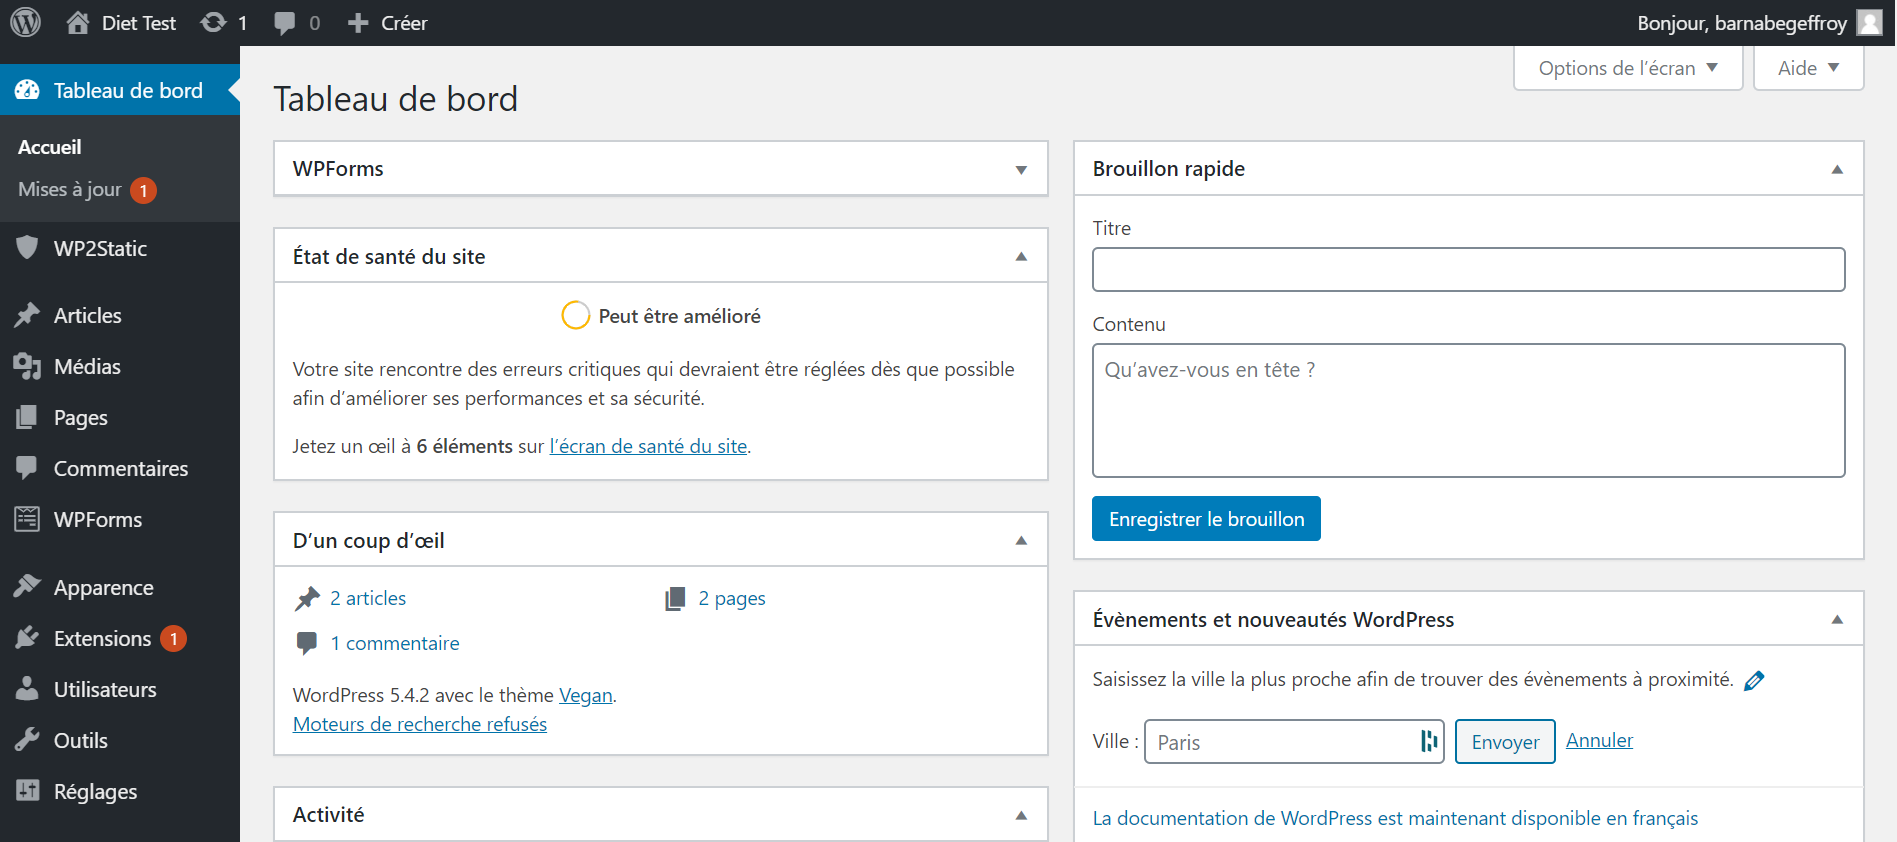
\includegraphics[width=\textwidth]{assets/wp.PNG}
    \end{center}
    \caption{Capture d'écran de l'interface de WordPress}
\end{figure}
Une contrainte s'ajoutait tout de même en utilisant WordPress. Le fait de n'avoir à aucun moment accès au code source et de dépendre d'extensions pouvant évoluer, ne plus être compatible était en effet un risque à éviter.

Il a donc été décidé de concevoir l'esthétique du site sur WordPress (affichage, thème, polices, images). La partie technique (dynamisme, récupération des données) serait développée sur Jekyll.

\subsection{Jekyll}
Jekyll est un générateur de site statique\footnote{Une page web statique est une page web dont le contenu ne varie pas en fonction des caractéristiques de la demande.}. Ce logiciel permet de générer facilement une architecture web convaincante. Jekyll 

\section{Déploiement sur Internet}


\section{Détails techniques}